% Options for packages loaded elsewhere
\PassOptionsToPackage{unicode}{hyperref}
\PassOptionsToPackage{hyphens}{url}
\PassOptionsToPackage{dvipsnames,svgnames,x11names}{xcolor}
%
\documentclass[
  letterpaper,
  DIV=11,
  numbers=noendperiod]{scrartcl}

\usepackage{amsmath,amssymb}
\usepackage{iftex}
\ifPDFTeX
  \usepackage[T1]{fontenc}
  \usepackage[utf8]{inputenc}
  \usepackage{textcomp} % provide euro and other symbols
\else % if luatex or xetex
  \usepackage{unicode-math}
  \defaultfontfeatures{Scale=MatchLowercase}
  \defaultfontfeatures[\rmfamily]{Ligatures=TeX,Scale=1}
\fi
\usepackage{lmodern}
\ifPDFTeX\else  
    % xetex/luatex font selection
\fi
% Use upquote if available, for straight quotes in verbatim environments
\IfFileExists{upquote.sty}{\usepackage{upquote}}{}
\IfFileExists{microtype.sty}{% use microtype if available
  \usepackage[]{microtype}
  \UseMicrotypeSet[protrusion]{basicmath} % disable protrusion for tt fonts
}{}
\makeatletter
\@ifundefined{KOMAClassName}{% if non-KOMA class
  \IfFileExists{parskip.sty}{%
    \usepackage{parskip}
  }{% else
    \setlength{\parindent}{0pt}
    \setlength{\parskip}{6pt plus 2pt minus 1pt}}
}{% if KOMA class
  \KOMAoptions{parskip=half}}
\makeatother
\usepackage{xcolor}
\usepackage[margin=.5in]{geometry}
\setlength{\emergencystretch}{3em} % prevent overfull lines
\setcounter{secnumdepth}{5}
% Make \paragraph and \subparagraph free-standing
\ifx\paragraph\undefined\else
  \let\oldparagraph\paragraph
  \renewcommand{\paragraph}[1]{\oldparagraph{#1}\mbox{}}
\fi
\ifx\subparagraph\undefined\else
  \let\oldsubparagraph\subparagraph
  \renewcommand{\subparagraph}[1]{\oldsubparagraph{#1}\mbox{}}
\fi

\usepackage{color}
\usepackage{fancyvrb}
\newcommand{\VerbBar}{|}
\newcommand{\VERB}{\Verb[commandchars=\\\{\}]}
\DefineVerbatimEnvironment{Highlighting}{Verbatim}{commandchars=\\\{\}}
% Add ',fontsize=\small' for more characters per line
\usepackage{framed}
\definecolor{shadecolor}{RGB}{241,243,245}
\newenvironment{Shaded}{\begin{snugshade}}{\end{snugshade}}
\newcommand{\AlertTok}[1]{\textcolor[rgb]{0.68,0.00,0.00}{#1}}
\newcommand{\AnnotationTok}[1]{\textcolor[rgb]{0.37,0.37,0.37}{#1}}
\newcommand{\AttributeTok}[1]{\textcolor[rgb]{0.40,0.45,0.13}{#1}}
\newcommand{\BaseNTok}[1]{\textcolor[rgb]{0.68,0.00,0.00}{#1}}
\newcommand{\BuiltInTok}[1]{\textcolor[rgb]{0.00,0.23,0.31}{#1}}
\newcommand{\CharTok}[1]{\textcolor[rgb]{0.13,0.47,0.30}{#1}}
\newcommand{\CommentTok}[1]{\textcolor[rgb]{0.37,0.37,0.37}{#1}}
\newcommand{\CommentVarTok}[1]{\textcolor[rgb]{0.37,0.37,0.37}{\textit{#1}}}
\newcommand{\ConstantTok}[1]{\textcolor[rgb]{0.56,0.35,0.01}{#1}}
\newcommand{\ControlFlowTok}[1]{\textcolor[rgb]{0.00,0.23,0.31}{#1}}
\newcommand{\DataTypeTok}[1]{\textcolor[rgb]{0.68,0.00,0.00}{#1}}
\newcommand{\DecValTok}[1]{\textcolor[rgb]{0.68,0.00,0.00}{#1}}
\newcommand{\DocumentationTok}[1]{\textcolor[rgb]{0.37,0.37,0.37}{\textit{#1}}}
\newcommand{\ErrorTok}[1]{\textcolor[rgb]{0.68,0.00,0.00}{#1}}
\newcommand{\ExtensionTok}[1]{\textcolor[rgb]{0.00,0.23,0.31}{#1}}
\newcommand{\FloatTok}[1]{\textcolor[rgb]{0.68,0.00,0.00}{#1}}
\newcommand{\FunctionTok}[1]{\textcolor[rgb]{0.28,0.35,0.67}{#1}}
\newcommand{\ImportTok}[1]{\textcolor[rgb]{0.00,0.46,0.62}{#1}}
\newcommand{\InformationTok}[1]{\textcolor[rgb]{0.37,0.37,0.37}{#1}}
\newcommand{\KeywordTok}[1]{\textcolor[rgb]{0.00,0.23,0.31}{#1}}
\newcommand{\NormalTok}[1]{\textcolor[rgb]{0.00,0.23,0.31}{#1}}
\newcommand{\OperatorTok}[1]{\textcolor[rgb]{0.37,0.37,0.37}{#1}}
\newcommand{\OtherTok}[1]{\textcolor[rgb]{0.00,0.23,0.31}{#1}}
\newcommand{\PreprocessorTok}[1]{\textcolor[rgb]{0.68,0.00,0.00}{#1}}
\newcommand{\RegionMarkerTok}[1]{\textcolor[rgb]{0.00,0.23,0.31}{#1}}
\newcommand{\SpecialCharTok}[1]{\textcolor[rgb]{0.37,0.37,0.37}{#1}}
\newcommand{\SpecialStringTok}[1]{\textcolor[rgb]{0.13,0.47,0.30}{#1}}
\newcommand{\StringTok}[1]{\textcolor[rgb]{0.13,0.47,0.30}{#1}}
\newcommand{\VariableTok}[1]{\textcolor[rgb]{0.07,0.07,0.07}{#1}}
\newcommand{\VerbatimStringTok}[1]{\textcolor[rgb]{0.13,0.47,0.30}{#1}}
\newcommand{\WarningTok}[1]{\textcolor[rgb]{0.37,0.37,0.37}{\textit{#1}}}

\providecommand{\tightlist}{%
  \setlength{\itemsep}{0pt}\setlength{\parskip}{0pt}}\usepackage{longtable,booktabs,array}
\usepackage{calc} % for calculating minipage widths
% Correct order of tables after \paragraph or \subparagraph
\usepackage{etoolbox}
\makeatletter
\patchcmd\longtable{\par}{\if@noskipsec\mbox{}\fi\par}{}{}
\makeatother
% Allow footnotes in longtable head/foot
\IfFileExists{footnotehyper.sty}{\usepackage{footnotehyper}}{\usepackage{footnote}}
\makesavenoteenv{longtable}
\usepackage{graphicx}
\makeatletter
\def\maxwidth{\ifdim\Gin@nat@width>\linewidth\linewidth\else\Gin@nat@width\fi}
\def\maxheight{\ifdim\Gin@nat@height>\textheight\textheight\else\Gin@nat@height\fi}
\makeatother
% Scale images if necessary, so that they will not overflow the page
% margins by default, and it is still possible to overwrite the defaults
% using explicit options in \includegraphics[width, height, ...]{}
\setkeys{Gin}{width=\maxwidth,height=\maxheight,keepaspectratio}
% Set default figure placement to htbp
\makeatletter
\def\fps@figure{htbp}
\makeatother

\usepackage[sfdefault]{roboto}
\KOMAoption{captions}{tableheading}
\makeatletter
\@ifpackageloaded{tcolorbox}{}{\usepackage[skins,breakable]{tcolorbox}}
\@ifpackageloaded{fontawesome5}{}{\usepackage{fontawesome5}}
\definecolor{quarto-callout-color}{HTML}{909090}
\definecolor{quarto-callout-note-color}{HTML}{0758E5}
\definecolor{quarto-callout-important-color}{HTML}{CC1914}
\definecolor{quarto-callout-warning-color}{HTML}{EB9113}
\definecolor{quarto-callout-tip-color}{HTML}{00A047}
\definecolor{quarto-callout-caution-color}{HTML}{FC5300}
\definecolor{quarto-callout-color-frame}{HTML}{acacac}
\definecolor{quarto-callout-note-color-frame}{HTML}{4582ec}
\definecolor{quarto-callout-important-color-frame}{HTML}{d9534f}
\definecolor{quarto-callout-warning-color-frame}{HTML}{f0ad4e}
\definecolor{quarto-callout-tip-color-frame}{HTML}{02b875}
\definecolor{quarto-callout-caution-color-frame}{HTML}{fd7e14}
\makeatother
\makeatletter
\makeatother
\makeatletter
\makeatother
\makeatletter
\@ifpackageloaded{caption}{}{\usepackage{caption}}
\AtBeginDocument{%
\ifdefined\contentsname
  \renewcommand*\contentsname{Table of contents}
\else
  \newcommand\contentsname{Table of contents}
\fi
\ifdefined\listfigurename
  \renewcommand*\listfigurename{List of Figures}
\else
  \newcommand\listfigurename{List of Figures}
\fi
\ifdefined\listtablename
  \renewcommand*\listtablename{List of Tables}
\else
  \newcommand\listtablename{List of Tables}
\fi
\ifdefined\figurename
  \renewcommand*\figurename{Figure}
\else
  \newcommand\figurename{Figure}
\fi
\ifdefined\tablename
  \renewcommand*\tablename{Table}
\else
  \newcommand\tablename{Table}
\fi
}
\@ifpackageloaded{float}{}{\usepackage{float}}
\floatstyle{ruled}
\@ifundefined{c@chapter}{\newfloat{codelisting}{h}{lop}}{\newfloat{codelisting}{h}{lop}[chapter]}
\floatname{codelisting}{Listing}
\newcommand*\listoflistings{\listof{codelisting}{List of Listings}}
\makeatother
\makeatletter
\@ifpackageloaded{caption}{}{\usepackage{caption}}
\@ifpackageloaded{subcaption}{}{\usepackage{subcaption}}
\makeatother
\makeatletter
\@ifpackageloaded{tcolorbox}{}{\usepackage[skins,breakable]{tcolorbox}}
\makeatother
\makeatletter
\@ifundefined{shadecolor}{\definecolor{shadecolor}{rgb}{.97, .97, .97}}
\makeatother
\makeatletter
\makeatother
\makeatletter
\makeatother
\ifLuaTeX
  \usepackage{selnolig}  % disable illegal ligatures
\fi
\IfFileExists{bookmark.sty}{\usepackage{bookmark}}{\usepackage{hyperref}}
\IfFileExists{xurl.sty}{\usepackage{xurl}}{} % add URL line breaks if available
\urlstyle{same} % disable monospaced font for URLs
\hypersetup{
  pdftitle={From Contingency Table To Logistic Regression},
  pdfauthor={Andy Grogan-Kaylor},
  colorlinks=true,
  linkcolor={blue},
  filecolor={Maroon},
  citecolor={Blue},
  urlcolor={Blue},
  pdfcreator={LaTeX via pandoc}}

\title{From Contingency Table To Logistic Regression}
\usepackage{etoolbox}
\makeatletter
\providecommand{\subtitle}[1]{% add subtitle to \maketitle
  \apptocmd{\@title}{\par {\large #1 \par}}{}{}
}
\makeatother
\subtitle{With the French Skiiers Data}
\author{Andy Grogan-Kaylor}
\date{2023-09-26}

\begin{document}
\maketitle
\ifdefined\Shaded\renewenvironment{Shaded}{\begin{tcolorbox}[sharp corners, frame hidden, boxrule=0pt, borderline west={3pt}{0pt}{shadecolor}, enhanced, breakable, interior hidden]}{\end{tcolorbox}}\fi

\renewcommand*\contentsname{Table of contents}
{
\hypersetup{linkcolor=}
\setcounter{tocdepth}{3}
\tableofcontents
}
\hypertarget{the-data}{%
\section{The Data}\label{the-data}}

We use the French Skiiers data that we have used in other examples.

\begin{Shaded}
\begin{Highlighting}[]

\KeywordTok{use} \StringTok{"FrenchSkiiers.dta"}
\end{Highlighting}
\end{Shaded}

\hypertarget{contingency-table}{%
\section{Contingency Table}\label{contingency-table}}

\begin{Shaded}
\begin{Highlighting}[]

\KeywordTok{tabulate}\NormalTok{ Tx Outcome [}\KeywordTok{fweight}\NormalTok{ = Count]}
\end{Highlighting}
\end{Shaded}

\begin{verbatim}
Running C:\Users\agrogan\Desktop\GitHub\newstuff\categorical\from-contingency-t
> able-to-logistic-regression\profile.do . 

              |        Outcome
           Tx |   No Cold       Cold |     Total
--------------+----------------------+----------
      Placebo |       109         31 |       140 
Ascorbic Acid |       122         17 |       139 
--------------+----------------------+----------
        Total |       231         48 |       279 
\end{verbatim}

For the sake of teaching and exposition, I re-arrange the numbers
slightly.

\begin{longtable}[]{@{}lcc@{}}
\toprule\noalign{}
& Develop Outcome & Do Not Develop Outcome \\
\midrule\noalign{}
\endhead
\bottomrule\noalign{}
\endlastfoot
Exposed & a & b \\
Not Exposed & c & d \\
\end{longtable}

\begin{longtable}[]{@{}lcc@{}}
\toprule\noalign{}
& Cold & No Cold \\
\midrule\noalign{}
\endhead
\bottomrule\noalign{}
\endlastfoot
Ascorbic Acid & 17 (a) & 122 (b) \\
Placebo & 31 (c) & 109 (d) \\
\end{longtable}

\hypertarget{risk-r-and-risk-differences-rd}{%
\subsection{\texorpdfstring{Risk (\(R\)) and Risk Differences
(\(RD\))}{Risk (R) and Risk Differences (RD)}}\label{risk-r-and-risk-differences-rd}}

\(R = \frac{a}{a+b}\) (in Exposed)

\(RD =\)

\(\text{risk in exposed} - \text{risk in not exposed} =\)

\(a/(a+b) - c/(c+d) =\)

\((17/139) - (31/140) =\)

\(-.09912641\)

\begin{quote}
How do we talk about this \emph{risk difference}?
\end{quote}

\hypertarget{odds-ratios-or}{%
\subsection{\texorpdfstring{Odds Ratios
(\(OR\))}{Odds Ratios (OR)}}\label{odds-ratios-or}}

\begin{longtable}[]{@{}lcc@{}}
\toprule\noalign{}
& Develop Outcome & Do Not Develop Outcome \\
\midrule\noalign{}
\endhead
\bottomrule\noalign{}
\endlastfoot
Exposed & a & b \\
Not Exposed & c & d \\
\end{longtable}

\(OR =\)

\(\frac{\text{odds that exposed person develops outcome}}{\text{odds that unexposed person develops outcome}} =\)

\(\frac{\frac{a}{a+b} / \frac{b}{a+b}}{\frac{c}{c+d} / \frac{d}{c+d}} =\)

\(\frac{a/b}{c/d} =\)

\(\frac{ad}{bc} =\)

\((17 * 109)/(122 * 31) =\)

\(.4899526\)

\begin{quote}
How do we talk about this \emph{odds ratio}?
\end{quote}

\hypertarget{logistic-regression}{%
\section{Logistic Regression}\label{logistic-regression}}

As discussed, the formula for logistic regression is:

\[\ln \Big(\frac{p(\text{outcome})}{1-p(\text{outcome})} \Big) = \beta_0 + \beta_1 x\]

Here \(p(\text{outcome})\) is the probability of the outcome.

\(\frac{p(\text{outcome})}{1-p(\text{outcome})}\) is the \emph{odds} of
the outcome.

Hence,
\(\ln \Big(\frac{p(\text{outcome})}{1-p(\text{outcome})} \Big)\)\footnote{It
  is sometimes useful to think of the \emph{log odds} as a
  \emph{transformed dependent variable}. We have transformed the
  dependent variable so that it can be expressed as a linear function of
  the independent variables, e.g.: \(\beta_0 + \beta_1 x\)} is the
\emph{log odds} of the outcome.

\begin{tcolorbox}[enhanced jigsaw, colback=white, opacitybacktitle=0.6, opacityback=0, breakable, titlerule=0mm, arc=.35mm, colbacktitle=quarto-callout-tip-color!10!white, rightrule=.15mm, coltitle=black, title=\textcolor{quarto-callout-tip-color}{\faLightbulb}\hspace{0.5em}{The logistic regression equation has the desired functional form.}, left=2mm, leftrule=.75mm, bottomtitle=1mm, toptitle=1mm, bottomrule=.15mm, colframe=quarto-callout-tip-color-frame, toprule=.15mm]

The logistic regression equation is appropriate to reflect changes in
the probability of an outcome that can be either 1 or 0.

\begin{figure}[H]

{\centering 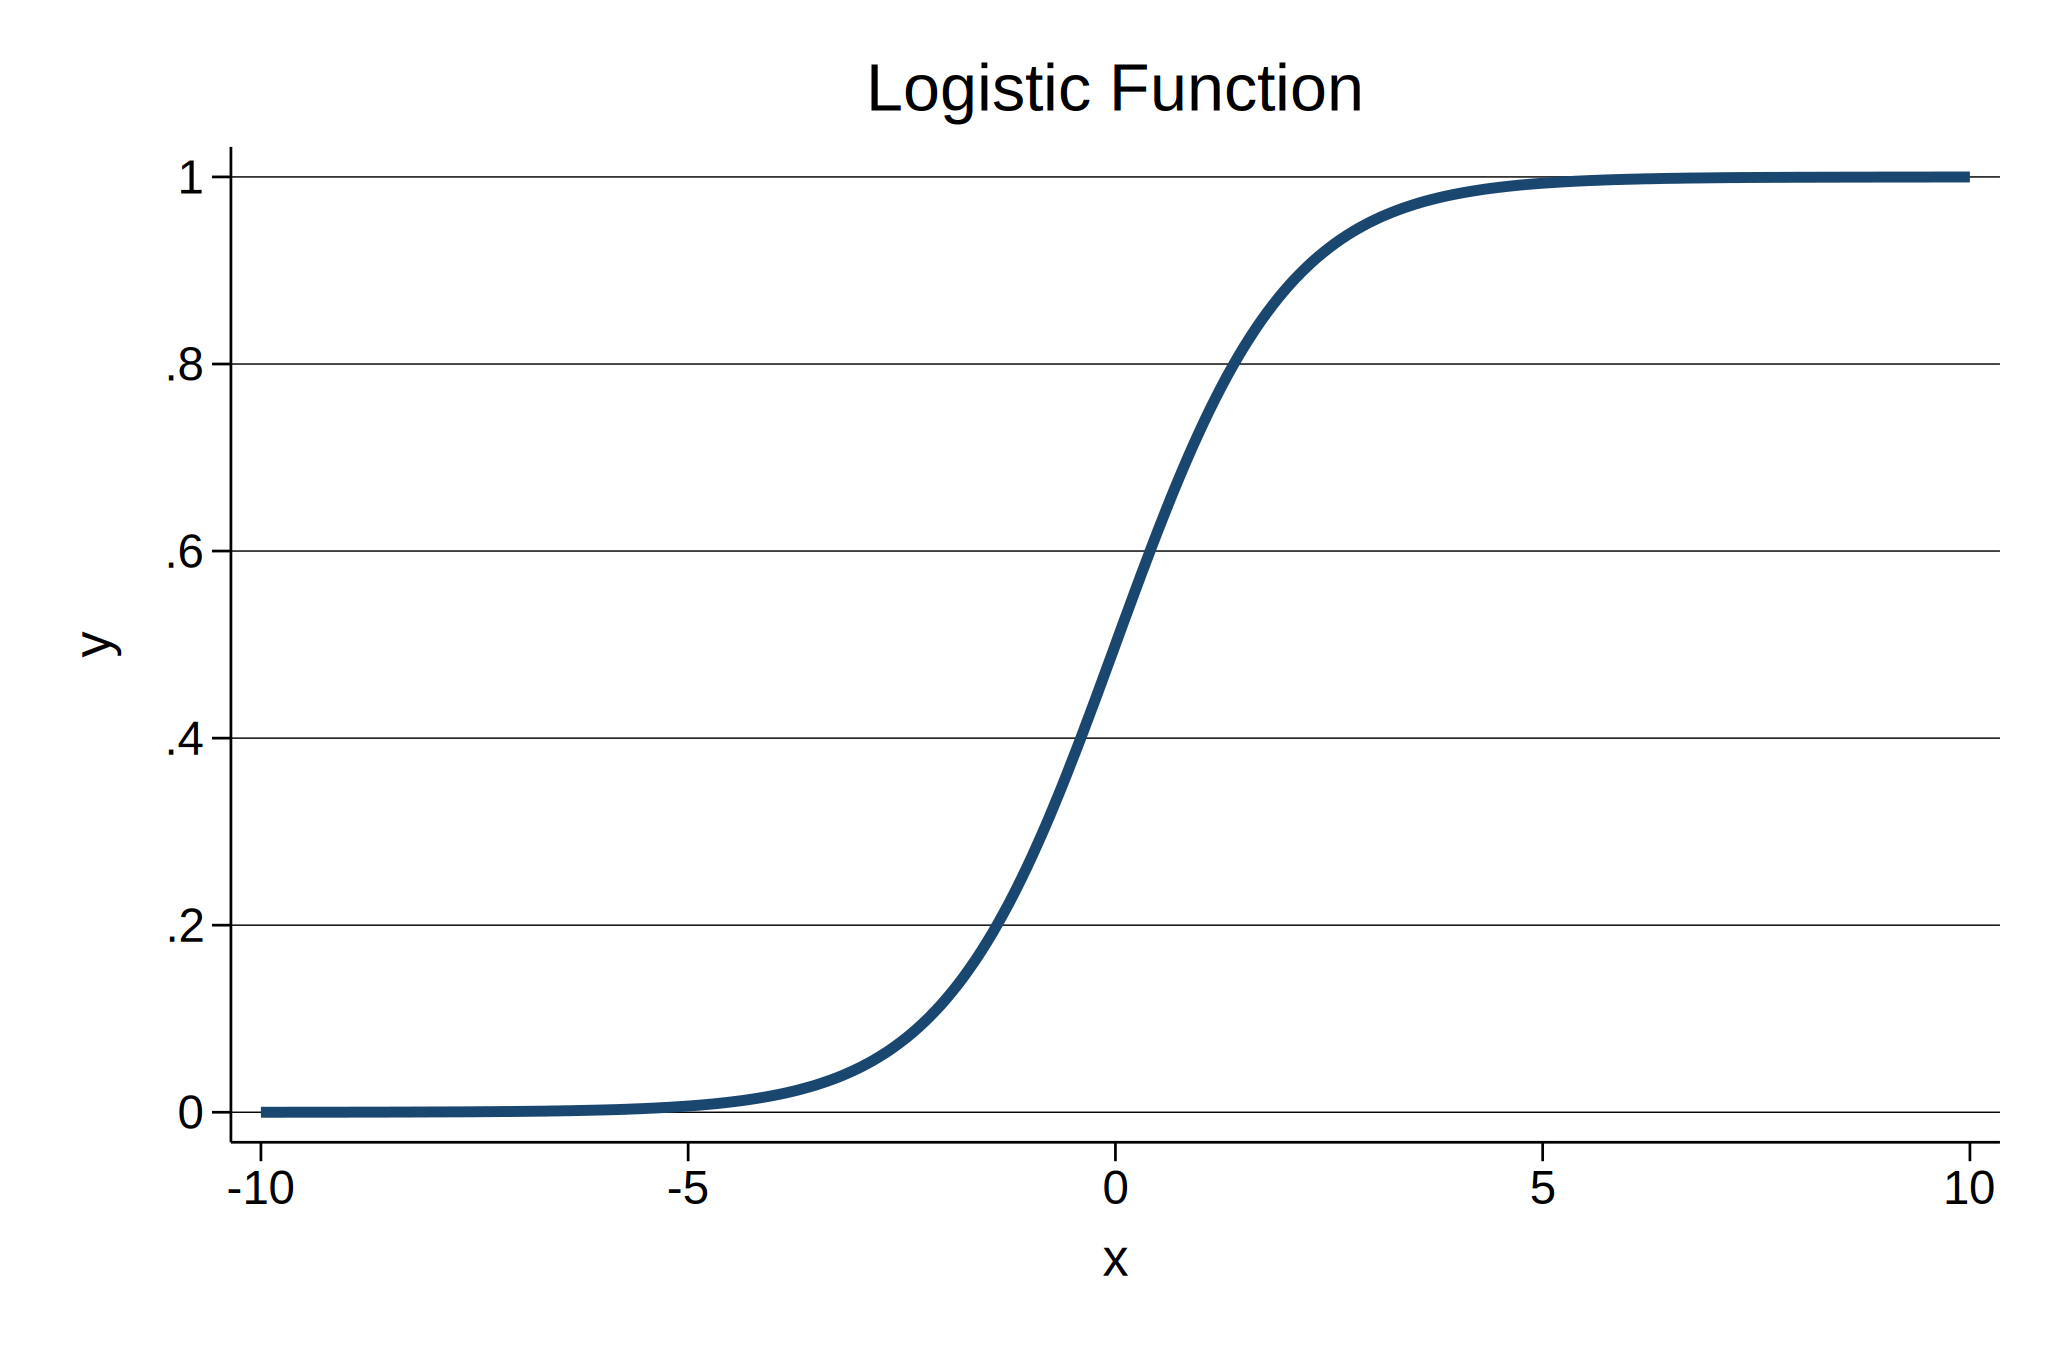
\includegraphics[width=0.5\textwidth,height=\textheight]{logistic.png}

}

\caption{Logistic Curve}

\end{figure}

\end{tcolorbox}

Logistic regression returns a \(\beta\) coefficient for each independent
variable \(x\).

These \(\beta\) coefficients can then be \emph{exponentiated} to obtain
\emph{odds ratios}: \(OR = e^{\beta}\)

\begin{tcolorbox}[enhanced jigsaw, colback=white, opacitybacktitle=0.6, opacityback=0, breakable, titlerule=0mm, arc=.35mm, colbacktitle=quarto-callout-tip-color!10!white, rightrule=.15mm, coltitle=black, title=\textcolor{quarto-callout-tip-color}{\faLightbulb}\hspace{0.5em}{Exponentiation ``undoes'' the logarithmic transformation.}, left=2mm, leftrule=.75mm, bottomtitle=1mm, toptitle=1mm, bottomrule=.15mm, colframe=quarto-callout-tip-color-frame, toprule=.15mm]

If \(\ln(y) = x\), then \(y = e^x\)

So, if \ldots{}
\(\ln \Big(\frac{p(\text{outcome})}{1-p(\text{outcome})}\Big) = \beta_0 + \beta_1 x\)
then
\(\frac{p(\text{outcome})}{1-p(\text{outcome})} = e^{\beta_0 + \beta_1 x} = e^{\beta_0} \times e^{\beta_1 x}\)

\end{tcolorbox}

\begin{quote}
We see that the odds ratio given by logistic regression,
\texttt{.4899526}, is the exact same as that given by manually
calculating the odds ratio from a contingency table.
\end{quote}

\begin{quote}
An advantage of logistic regression is that it can be extended to
multiple independent variables.
\end{quote}

\begin{Shaded}
\begin{Highlighting}[]

\KeywordTok{logit}\NormalTok{ Outcome Tx [}\KeywordTok{fweight}\NormalTok{ = Count], }\KeywordTok{or}
\end{Highlighting}
\end{Shaded}

\begin{verbatim}
Running C:\Users\agrogan\Desktop\GitHub\newstuff\categorical\from-contingency-t
> able-to-logistic-regression\profile.do . 

Iteration 0:  Log likelihood = -128.09195  
Iteration 1:  Log likelihood = -125.68839  
Iteration 2:  Log likelihood = -125.65611  
Iteration 3:  Log likelihood =  -125.6561  

Logistic regression                                     Number of obs =    279
                                                        LR chi2(1)    =   4.87
                                                        Prob > chi2   = 0.0273
Log likelihood = -125.6561                              Pseudo R2     = 0.0190

------------------------------------------------------------------------------
     Outcome | Odds ratio   Std. err.      z    P>|z|     [95% conf. interval]
-------------+----------------------------------------------------------------
          Tx |   .4899526   .1613519    -2.17   0.030      .256942    .9342712
       _cons |   .2844037   .0578902    -6.18   0.000     .1908418     .423835
------------------------------------------------------------------------------
Note: _cons estimates baseline odds.
\end{verbatim}

\begin{quote}
How do we talk about this \emph{odds ratio}? How would we talk about it
if it was \(> 1.0\)? \(> 2.0\)
\end{quote}



\end{document}
